% Presentación final · Torneo Itaú–FEN 2026 · Diego Ponce y Simón Canales
% Compilar con pdfLaTeX (TeXstudio). Necesita en la misma carpeta: fig5_curva_prueba.pdf y deterioro.pdf
\documentclass[aspectratio=169,11pt]{beamer}
\usepackage[utf8]{inputenc}
\usepackage[T1]{fontenc}
\usepackage[spanish,es-nodecimaldot]{babel}
\usepackage{lmodern}
\usepackage{tikz}
\usetikzlibrary{arrows.meta,positioning}

% ---------- estilo: Madrid + beaver (rojo y gris) ----------
\usetheme{Madrid}
\usecolortheme{beaver}
\setbeamertemplate{navigation symbols}{}
\setbeamertemplate{blocks}[rounded][shadow=true]
\setbeamerfont{title}{size=\Huge}
\setbeamerfont{subtitle}{size=\large,series=\bfseries}
% barra superior: sección actual en rojo (izquierda) y franja gris (derecha), como en el ejemplo
\setbeamercolor{section in head/foot}{bg=darkred,fg=white}
\setbeamercolor{subsection in head/foot}{bg=gray!20,fg=darkred}
\setbeamertemplate{headline}{\leavevmode\hbox{%
  \begin{beamercolorbox}[wd=.5\paperwidth,ht=2.5ex,dp=1.1ex,left]{section in head/foot}\hspace*{2ex}\small\insertsectionhead\end{beamercolorbox}%
  \begin{beamercolorbox}[wd=.5\paperwidth,ht=2.5ex,dp=1.1ex,right]{subsection in head/foot}\end{beamercolorbox}}}
\definecolor{azul}{RGB}{31,78,121}
\colorlet{rojo}{darkred}
\definecolor{gris}{RGB}{110,110,110}
\setbeamertemplate{itemize items}[circle]
% Las fuentes de cada cifra quedan en el código (\fuente{...}) y en Guia_Presentacion.pdf, pero no se muestran.
\newcommand{\fuente}[1]{}
\newcommand{\cifra}[2]{\begin{minipage}[t]{0.3\textwidth}\centering{\Huge\bfseries\color{darkred}#1}\\[1mm]{\small #2}\end{minipage}}

\title[¿Sube o baja el dólar mañana?]{¿Sube o baja el dólar mañana?}
\subtitle{Una ventaja real para predecir el USD/CLP\ldots\ que se agotó}
\author[D. Ponce y S. Canales]{Diego Ponce \and Simón Canales}
\institute[FEN U. de Chile]{Facultad de Economía y Negocios, Universidad de Chile}
\date[2 dic 2026]{Torneo Itaú--FEN · 2 de diciembre de 2026}

\begin{document}

% 1 ------------------------------------------------------------
\begin{frame}
\titlepage
\end{frame}

\section{La pregunta y el método}
% 2 ------------------------------------------------------------
\begin{frame}{La pregunta: ¿se puede ganar anticipando el dólar?}
\begin{itemize}\setlength\itemsep{4mm}
\item Cada día: comprar dólares, venderlos o quedarse fuera\\ {\small\color{gris}exposición de $-3$, $-1$, $0$, $+1$ o $+3$}
\item Ganar significa subir \textbf{más que el carry} y pagar los costos
\item Hay que vencer a tres referencias: no operar, comprar siempre y exposición fija
\end{itemize}
\fuente{bases del torneo; informe, ecuación (1), p.~11}
\end{frame}

% 3 ------------------------------------------------------------
\begin{frame}{La idea: Nueva York sigue operando cuando Chile ya cerró}
\centering
\begin{tikzpicture}[x=1cm,y=1cm,>=Stealth]
\draw[thick,gris] (0,0) -- (13,0);
\foreach \x/\t in {1/{9:00},4/{13:30},8/{18:00--19:00},12/{9:00 (día siguiente)}}
  {\draw[gris] (\x,0.15)--(\x,-0.15); \node[below,gris,font=\small] at (\x,-0.2) {\t};}
\node[above,align=center,font=\small] at (4,0.3) {\textbf{Cierra el peso}\\en Chile};
\node[above,align=center,font=\small] at (8,0.3) {\textbf{Cierra Nueva York}\\MXN, ZAR, BRL, DXY,\\EUR y S\&P~500};
\node[above,align=center,font=\small] at (12,0.3) {\textbf{Abre el peso}\\¿se ajusta?};
\fill[azul!15] (4,-0.08) rectangle (8,0.08);
\node[azul,font=\small\bfseries] at (6,-0.9) {horas que el peso aún no incorporó};
\draw[->,very thick,azul] (8.3,1.6) to[bend left=25] node[above,font=\small]{señal NY} (11.7,1.6);
\end{tikzpicture}
\vspace{6mm}
\begin{itemize}
\item Supuesto del torneo: todo cierra a la misma hora
\end{itemize}
\fuente{informe, Tabla 2 (p.~9) y Sección 1; mentoría del 6 de noviembre}
\end{frame}

% 4 ------------------------------------------------------------
\begin{frame}{De la señal a la apuesta: más seguros, apuesta más grande}
\centering
\begin{tikzpicture}[>=Stealth,node distance=1.2cm,
  caja/.style={draw=azul,thick,rounded corners,align=center,minimum height=1.4cm,text width=3.3cm,font=\small}]
\node[caja] (a) {\textbf{Señal NY}\\lo que pasó en NY\\después del cierre};
\node[caja,right=of a] (b) {\textbf{Probabilidad}\\de que el dólar suba\\{\color{gris}logit calibrado}};
\node[caja,right=of b] (c) {\textbf{Tamaño}\\$-3,\,-1,\,0,\,+1,\,+3$\\{\color{gris}Kelly fraccional}};
\draw[->,thick,azul] (a)--(b); \draw[->,thick,azul] (b)--(c);
\end{tikzpicture}
\vspace{8mm}
\begin{itemize}
\item Si la ventaja no paga el riesgo y el costo: \textbf{no se apuesta}
\end{itemize}
\fuente{informe, ecuaciones (2) a (5), pp.~11--12}
\end{frame}

% 5 ------------------------------------------------------------
\begin{frame}{Para no engañarnos: el examen se rinde una sola vez}
\centering
\begin{tikzpicture}[x=1cm,y=1cm]
\fill[azul!25] (0,0) rectangle (6.5,0.8);   \node[font=\small] at (3.25,0.4) {Entrenar · 2004--2019};
\fill[azul!55] (6.5,0) rectangle (9.5,0.8); \node[font=\small,white] at (8,0.4) {Elegir · 2020--23};
\fill[rojo!75] (9.5,0) rectangle (12.4,0.8);\node[font=\small,white] at (10.95,0.4) {Prueba · 2024--26};
\fill[gris!50] (12.4,0) rectangle (13.2,0.8);
\node[font=\scriptsize,align=center] at (13.6,-0.5) {en vivo\\13 nov--1 dic};
\node[font=\scriptsize,align=center,rojo] at (10.95,-0.5) {una sola corrida\\6 de noviembre};
\end{tikzpicture}
\vspace{5mm}
\begin{itemize}\setlength\itemsep{2mm}
\item Cada año se predice solo con datos del pasado
\item Modelo congelado y registrado en GitHub \textbf{antes} de mirar la prueba
\item 15 experimentos anotados, también los descartados
\end{itemize}
\fuente{informe, Tabla 1 (p.~8), Sección 4.3 y Tabla 17 (p.~34)}
\end{frame}

\section{Resultados}
% 6 ------------------------------------------------------------
\begin{frame}{Hasta 2023, la señal funcionaba}
\centering\vspace{4mm}
\cifra{12,1\%}{retorno anual neto\\{\color{gris}comprar siempre: 0,4\%}}\hfill
\cifra{0,92}{Sharpe}\hfill
\cifra{$-10$\%}{pérdida máxima\\{\color{gris}comprar siempre: $-35$\%}}
\vspace{10mm}
\begin{itemize}
\item Le gana a no operar con significancia ($p=0{,}012$)
\item A comprar siempre, por mucho, pero sin significancia ($p=0{,}08$)
\end{itemize}
\fuente{informe, Tabla 7 (p.~19) y Tabla 8 (p.~20); validación 2020--2023}
\end{frame}

% 7 ------------------------------------------------------------
\begin{frame}{En la prueba, perdimos plata}
\begin{columns}[c]
\column{0.62\textwidth}
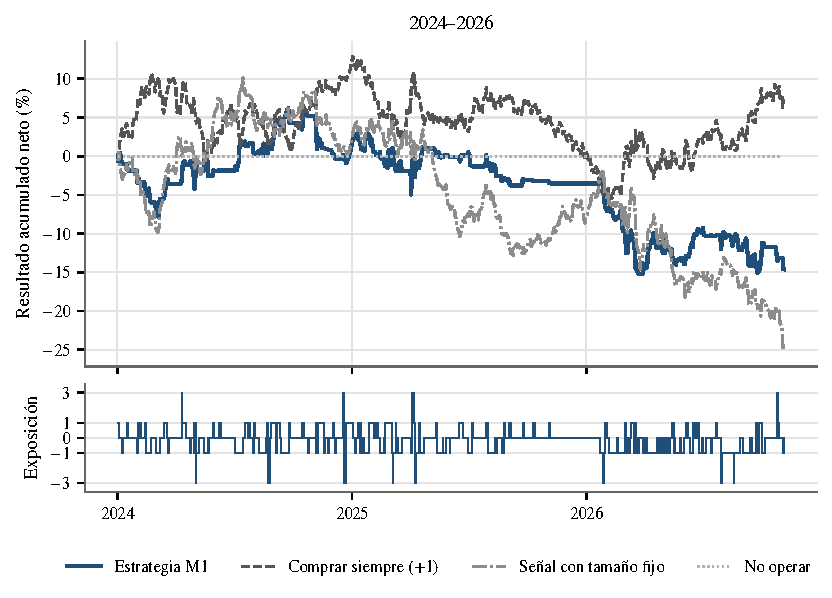
\includegraphics[width=\linewidth]{fig5_curva_prueba.pdf}
\column{0.36\textwidth}
{\Huge\bfseries\color{rojo}$-5{,}1$\%}\\{\small al año · Sharpe $-0{,}54$}\\[5mm]
{\Large\bfseries $+2{,}7$\%}\\{\small comprar siempre}\\[5mm]
{\small La señal ya no anticipa la dirección\\{\color{gris}Clark-West $p=0{,}52$}}
\end{columns}
\fuente{informe, Tabla 9 y Figura 3 (pp.~21--22); 716 jornadas, ene.~2024 -- nov.~2026}
\end{frame}

% 8 ------------------------------------------------------------
\begin{frame}{Por qué: la señal de Nueva York se fue apagando}
\centering
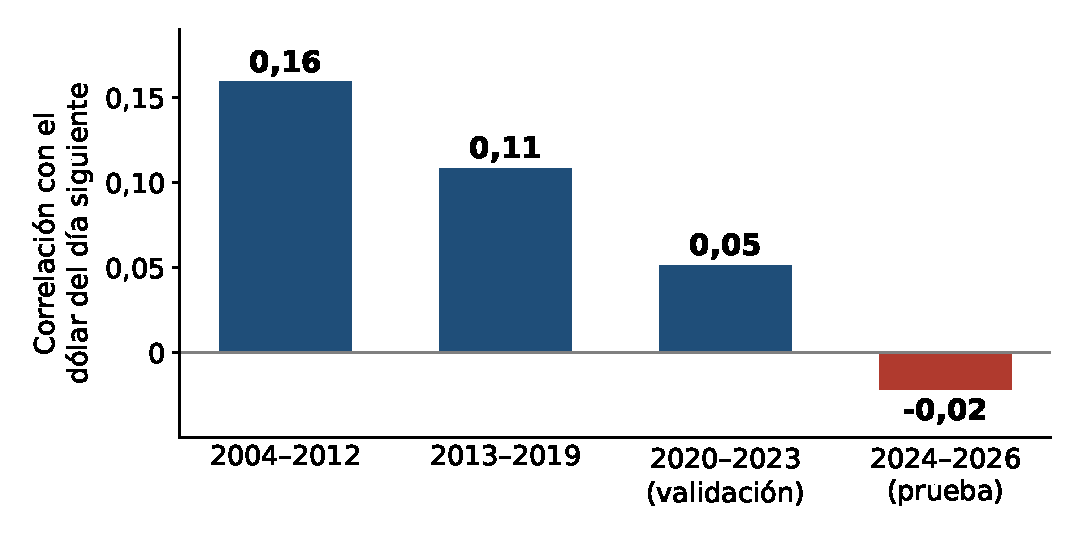
\includegraphics[width=0.78\textwidth]{deterioro.pdf}
\fuente{informe, Tabla 12 (p.~23)}
\end{frame}

\section{Lecciones}
% 9 ------------------------------------------------------------
\begin{frame}{No fue mala suerte, y había alertas antes de la prueba}
\begin{itemize}\setlength\itemsep{4mm}
\item Si la ventaja siguiera, ver este resultado tendría $\approx$1\% de probabilidad
\item Alertas registradas \textbf{antes} de mirar:
  \begin{itemize}\setlength\itemsep{1mm}
  \item entrenado solo desde 2013, el modelo ya no ganaba ($-0{,}2$\%)
  \item la ventaja vivía en horas en que el peso no se transa
  \item el Sharpe deflactado no llegaba al umbral (0,65)
  \end{itemize}
\end{itemize}
\fuente{informe, Sección 9 (p.~31), Sección 6.2 (p.~23) y Sección 6.1.4 (p.~20)}
\end{frame}

% 10 -----------------------------------------------------------
\begin{frame}{Saber cuándo no apostar limitó la pérdida}
\centering\vspace{4mm}
\cifra{54\%}{de los días\\sin posición}\hfill
\cifra{13}{días con apuesta\\máxima en 3 años}\hfill
\cifra{$-5{,}1$\%}{nuestra regla\\{\color{gris}apostando siempre 1: $-8{,}9$\%}}
\vspace{10mm}
\begin{itemize}
\item La pérdida vino de los días de apuesta chica, no de las grandes
\end{itemize}
\fuente{informe, Tabla 9 (p.~21) y Tabla 11 (p.~23)}
\end{frame}

% 11 -----------------------------------------------------------
\begin{frame}{Qué haríamos distinto}
\begin{itemize}\setlength\itemsep{4mm}
\item Una regla de \textbf{apagado}, fijada antes: si la señal deja de predecir, salir
\item Tomar todos los precios a una \textbf{misma hora} (datos intradía)
\item Estudiar el mercado \textbf{offshore}, que opera de noche
\item Monitoreo en vivo: esperamos un resultado cercano a cero
\end{itemize}
\fuente{informe, Sección 9, Extensiones (p.~31) y Sección 8 (p.~30)}
\end{frame}

% 12 -----------------------------------------------------------
\begin{frame}{En resumen}
\begin{enumerate}\setlength\itemsep{6mm}
\item {\large Lo que pasa en Nueva York después del cierre chileno anticipaba el dólar de mañana, pero esa ventaja se agotó}
\item {\large Como congelamos el modelo antes de mirar, el resultado, aunque negativo, es creíble}
\item {\large Saber cuándo no apostar fue lo que mejor resistió}
\end{enumerate}
\vfill\centering{\Large\color{azul}Gracias}
\end{frame}

\end{document}
